\documentclass[tikz,dvipsnames]{standalone}
\usepackage{pgfplots}
\usetikzlibrary{backgrounds}
\usetikzlibrary{calc,positioning,shapes.misc,fillbetween}

\begin{document}
 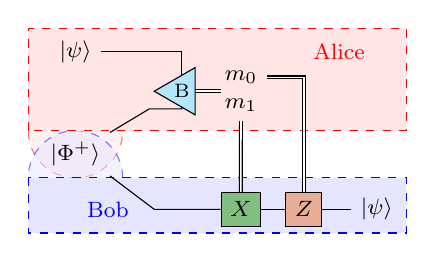
\begin{tikzpicture}[
    show background rectangle,
    tight background=0,
    font=\footnotesize,
    background rectangle/.style={fill=white},
 ]
    \coordinate (E) at (0,1.9);
    \coordinate (F) at (0,0.6);
    \coordinate (G) at (1,-0.1);

    \draw[name path=Al,red,fill=Red!10,opacity=0.5,dashed,rounded corners=6pt] ($(F)+(0,+0.3)$) circle (0.6);
    \draw[name path=Bo,blue,fill=Blue!10,opacity=0.5,dashed,rounded corners=3pt] ($(F)+(0,-0.3)$) circle (0.6);
    
    \draw[dashed,anchor=east,red,fill=red!10] 
    (F)++(-0.6,0.3) rectangle (4.2,2.2) (E)++(3.8,0)
    node[opacity=1] {Alice};
    \draw[dashed,anchor=east,blue,fill=blue!10] 
    (F)++(-0.6,-0.3) rectangle (4.2,-0.4) (F)++(0.8,-0.7)
    node[opacity=1] {Bob};
    
    \node at (E) (EE) {$|\psi\rangle$};
    \node at (F) (FF) {$|\Phi^+\rangle$};
    
    \coordinate (P) at ($(E)+(1,-0.5)$);
    \coordinate (Q) at ($(P)+(0.35,0)$);
    \draw (EE) -| ($(Q)+(0,-0.1)$);
    \draw (FF.north east) -- ++ (0.5,+0.3) -| ($(Q)+(0,-0.1)$);
    
     
    \node[xshift=10pt,yshift=+5pt] at ($(Q)+(0.4,0)$) (M0) {$m_0$};
    \node[xshift=10pt,yshift=-5pt] at ($(Q)+(0.4,0)$) (M1) {$m_1$};
    \draw[double] (Q) -- ++(0.5,0);
    \filldraw[fill=cyan!30] (P) -- ++(30:0.6) -- ++(270:0.6) -- cycle;
    \node at (Q) {\scriptsize B};
        
    \node[fill=Green!50   ,draw] at ($(G)+(1.1,0)$) (X) {$X$};
    \node[fill=BrickRed!30,draw] at ($(G)+(1.9,0)$) (Z) {$Z$};
    \draw[double] (M0) -| (Z);
    \draw[double] (M1.south) -- (X);
    \draw (X) -- (Z) -- ++(0.6,0) node[anchor=west] {$|\psi\rangle$};
    \draw (FF.south east) -- (G)-- (X.west);
       
    
    
    

\end{tikzpicture}
\end{document}
